\documentclass[10pt,letterpaper]{IEEEtran}
%\usepackage{citesort}
\usepackage{color}
\usepackage{url}
\usepackage[latin9]{inputenc}
\usepackage{epstopdf}
\usepackage{amsthm}
\usepackage{amsmath}
\usepackage{amsthm}
\usepackage{amssymb}
\usepackage{graphicx}
\usepackage{subfigure}
\usepackage{wrapfig}
\usepackage{algorithmic}
\usepackage{algorithm}
\usepackage{mathrsfs}
\usepackage{float}
\usepackage{mathtools}
\usepackage{tabulary}
\usepackage{booktabs}
\usepackage{caption}

\PassOptionsToPackage{bookmarks={false}}{hyperref}

\IEEEoverridecommandlockouts
%\usepackage{cite}
%\usepackage{amsmath,amssymb,amsfonts}
%\usepackage{algorithmic}
%\usepackage{graphicx}
%\usepackage{epstopdf}
%\usepackage{textcomp}
%\usepackage{xcolor}
%\usepackage{url}
%\usepackage{subcaption}
%\usepackage{subfigure}

\setlength{\topmargin}{-0.5in} \setlength{\headheight}{0in} \setlength{\headsep}{0in}
\setlength{\textheight}{9.6in}

\setlength{\oddsidemargin}{-0.375in}
\setlength{\evensidemargin}{-0.375in}
\setlength{\textwidth}{7.0in}


\def\BibTeX{{\rm B\kern-.05em{\sc i\kern-.025em b}\kern-.08em
   T\kern-.1667em\lower.7ex\hbox{E}\kern-.125emX}}

%\usepackage[ruled,vlined]{algorithm2e}
%\include{pythonlisting}
%\renewcommand{\algorithmicrequire}{\textbf{Input:}}

%\renewcommand{\algorithmicensure}{\textbf{Output:}}

\newcommand{\N}{\mathbb{N}}



\newcommand{\protocol}{{\tt{HybridCache}}}
\newcommand{\comment}[1]{ }

\DeclareMathOperator*{\argmin}{argmin}
\captionsetup[table]{
  labelsep=newline,
  justification=centering,
  singlelinecheck=false,
}

\newcommand\subparagraph{%
  \@startsection{subparagraph}{0}
  {\parindent}
  {0ex \@plus 0ex \@minus 0ex}
  {-1em}
  {\normalfont\normalsize\bfseries}}
\makeatother

\usepackage{titlesec}
\titlespacing*{\section}
{0pt}{1.2ex}{0ex} % indent; before subsec; after sub
\titlespacing*{\subsection}
{0pt}{1ex}{0ex}  % indent; before subsec; after sub
\titlespacing*{\subsubsection}
{0pt}{0ex}{0ex} % indent; before subsec; after sub

\begin{document}


\title{The Title of Your Project}

\author{ECE/CS 478 Class Project~\\
Author 1's Name, Author 2's Name, Author 3's Name~\\
\small Oregon State University, Corvallis, OR, USA, {author1,author2,author3}@oregonstate.edu \\
}

\maketitle
\thispagestyle{plain}
\pagestyle{plain}

%\begin{abstract}
%\input{files/tex/Abstract}
%\end{abstract}

%\begin{IEEEkeywords}
%Index term 1, index term 2, etc.
%\end{IEEEkeywords}

\section{Introduction}
Introduction text comes here. Whatever I type here, appears.

\section{Background}
\label{sec:background}
\input{files/tex/Background}


\section{Your next Section}
\label{sec:xxx}
%% how to cite a prior work
When citing some other reference, make sure to use the right method. Example, the authors of~\cite{hybridcache20tirupathi} have introduced xxx



\section{Your next next Section}
\label{sec:xxxx}
%%% how use itemize
When needing to itemize text, make sure to use:
\begin{itemize}
    \item \textbf{Method 1:}  This method is xxx
    \item \textbf{Method 2:}  This method is xxx
\end{itemize}



\section{Your third next Section (if needed)}
\label{sec:xxxxxx}
When you need to add an equation, you should use:
\begin{equation}
   x=y
\label{eq:ex}
\end{equation}
and then reference to the equation in the text using Equation~\eqref{eq:ex}.

When you need to include a table, you should use:
\begin{table}[ht]
\centering % centering table
\caption{\small Table title goes here} %title of the table
\begin{tabular}{c rrrr} % creating eight columns
\hline %inserting double-line
  & A & B & C\\
\hline % inserts single-line
One & 3409 & 42.3m & 50\\ % Entering row contents
Two & 1042 & 136.8m & 25\\
Three & 1004 & 150.8m & 25\\ % [1ex] adds vertical space
\hline % inserts single-line
Total & 6097 & 212.5m & 130\\
\hline % inserts single-line
\end{tabular}
\label{tab:hresult}
\end{table}

and then reference the table using Table~\ref{tab:hresult}.


\section{Your fourth next section (if needed)}
\label{sec:evaluation}
%% below is an example of how to insert a figure in the txt
\begin{figure}[ht]
\centerline{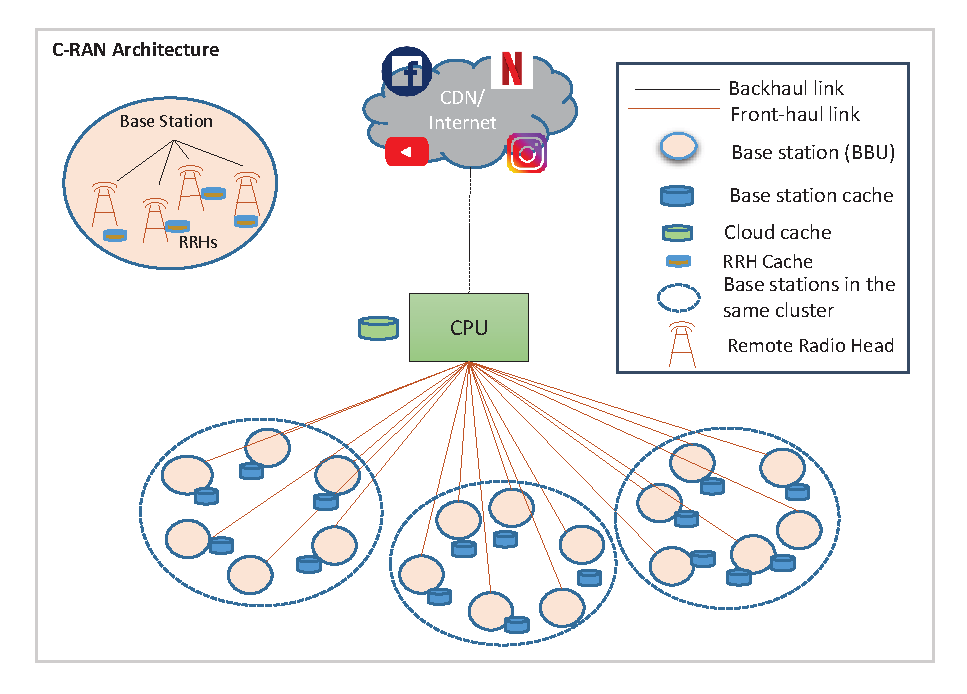
\includegraphics[width=0.8\linewidth]{files/figures/Architecture.eps}}
\caption{Sample figure caption.}
\label{fig0}
\end{figure}

When referencing a figure, make sure to call it within the text using its label. Here is an example: Figure~\ref{fig0} depicts... 


\section{Conclusion}
\label{sec:conclusion}
\input{files/tex/Conclusion}

\section{Individual Contributions}
\label{sec:contributions}
Each member contribution should be included here.


\bibliographystyle{IEEEtran}
\bibliography{References}
%\bibliographystyle{main}


\end{document}
